\documentclass[conference]{IEEEtran}
\IEEEoverridecommandlockouts
\usepackage{cite,amsmath,graphicx,booktabs,url,xcolor}
\usepackage[hidelinks]{hyperref}
\def\BibTeX{{\rm B\kern-.05em{\sc i\kern-.025em b}\kern-.08em T\kern-.1667em\lower.7ex\hbox{E}\kern-.125emX}}

\begin{document}

\title{Beyond Repetition: Language Models Over-Attribute\\Unresolved Communication in Everyday Dialogue}

\author{\IEEEauthorblockN{Anonymous Submission}
\IEEEauthorblockA{Double-blind review}}

\maketitle

\begin{abstract}
Proposals to infer cognitive health from everyday human--AI interaction presuppose that the model
reads the interaction correctly: that it can tell a communication problem that is still open from a
repetition that is perfectly ordinary. We test that presupposition. We build a corpus of 120
scenario families, each realised in a $2\times2$ crossing of surface repetition against repair
state, matched within family on turn count, length, question marks and a character-identical final
sentence, so that repetition carries no information about the label by construction. Across
Gemma-3 (4B, 12B) and Qwen2.5-7B we find that the judgement is at chance
(paired accuracy $0.54$--$0.60$, all $p>0.2$), that a character $n$-gram baseline beats every model
($0.76$), that at a pre-registered layer the residual stream adds nothing over a $19$-feature
surface model, and that no intervention among $40$ arms---dense axis, component swap, SAE feature
ablation and donor transplant, against matched random-direction, competing-axis and
random-feature controls---produces any selectivity (largest gap $0.15$). On $97$ ordinary human
conversations---97 of which are annotated as having nothing open---the three models label $86\%$,
$100\%$ and $84\%$ respectively as containing an unresolved problem,
irrespective of whether the segment repeats at all. This is a mechanism audit of a
prerequisite, not a measurement of cognition; the construct is an observable interaction state and
nothing here speaks to cognitive status.
\end{abstract}

\begin{IEEEkeywords}
conversational repair, interpretability, sparse autoencoders, dialogue evaluation, responsible AI
\end{IEEEkeywords}

\section{Introduction}
\label{sec:intro}

There is growing interest in using everyday human--AI conversation as a substrate for cognitive
health research: the interaction is longitudinal, naturalistic and already instrumented. Any such
programme rests on a prerequisite that is rarely tested. Before a conversational signal can inform
anything about a person, the model producing or scoring that conversation has to interpret the
interaction evidence correctly---and in particular it has to distinguish a communication problem
that is \emph{still open} from surface behaviour that merely resembles one.

Repetition is the sharpest case. A user who repeats themselves may be re-asking a question that was
never answered; they may equally be reading back a confirmation the assistant explicitly requested.
The words look alike; the interaction states are opposite. Recent work finds that automatic
annotation of conversational repair leans on lexical cues and neglects context \cite{ngo2026}. If
models inherit that bias, then an interaction-derived signal will track how often someone repeats
themselves rather than whether anything is actually wrong---which, for a population that repeats
more for entirely benign reasons, is precisely the wrong failure mode.

We evaluate Gemma-3~\cite{gemma3} at 4B and 12B and Qwen2.5-7B~\cite{qwen25}.

We ask two questions. \textbf{RQ-A}: with repetition decorrelated from repair state by
construction, is the interaction state recoverable---behaviourally, and from the residual stream?
\textbf{RQ-B}: do interventions on residual directions and sparse-autoencoder (SAE) features change
that context judgement \emph{specifically}, or only induce a generalized ``ask more questions''
tendency?

Our contributions are: (i) a controlled corpus in which surface repetition provably carries no
label information, with the leakage that survives measured rather than assumed; (ii) the finding
that three instruction-tuned models over-attribute unresolved communication to $84$--$100\%$ of
ordinary human dialogue; (iii) a negative mechanistic result with matched controls across $40$
intervention arms; and (iv) two acceptance checks---causal reachability and SAE
reconstruction-damage---each of which, omitted, would have produced a confident false finding.

\section{Related work}
\label{sec:related}

\textbf{Persona and behavioural directions.} Linear directions in the residual stream track
assistant persona and can be manipulated at inference time \cite{assistantaxis}. We ask the
adjacent question: not how the model represents \emph{itself}, but how it represents the
\emph{user's interaction evidence}, and whether that representation is used.

\textbf{SAE features and clarification.} Sparse features associated with clarification behaviour
can be identified and steered \cite{clarifysae}. Our contribution is the selectivity test: whether
such an intervention distinguishes contexts that need repair from contexts that do not, rather than
raising clarification everywhere.

\textbf{Repair annotation and lexical dependence.} Automatic repair annotation has been shown to
depend on lexical form and to under-use context \cite{ngo2026}. We supply the lexically matched
counterfactuals, the internal representation, and the controlled feature interventions.

\textbf{SAEs in clinical text.} SAEs have been applied to medical report generation and clinical
text \cite{maira2sae,cast}. Applying an SAE to a new domain is not by itself a contribution; what
is missing, and what we provide, is a causal test of whether the identified features are used.

\section{A repetition-controlled repair corpus}
\label{sec:data}

\subsection{Design}
The unit is a short task-oriented dialogue that begins and ends on a user turn. A \emph{family} is
one scenario realised in four conditions, a full crossing of surface repetition
(\textsc{rep}/\textsc{norep}) against repair state (\textsc{unres}/\textsc{res}). Because the
crossing is complete, a classifier keying on repetition alone scores exactly chance.

A positive (\textsc{unres}) label requires quotable evidence of exactly one of:
\emph{unanswered question}, \emph{contradiction}, or \emph{ambiguous reference}. A single
repetition, disfluency, brevity, politeness or stated age is never sufficient. Health, memory, age
and diagnosis wording is forbidden anywhere in the text, so neither model nor annotator can
shortcut from a health cue to the label.

Within a family we hold constant: domain, entities and task goal; turn count and speaker sequence;
total length to within $\pm18\%$; question-mark count to within one; and---critically---the
\textbf{final sentence of the last user turn, character-identical across all four conditions}. That
sentence is where representations are read, so it must not itself carry the label. In $62\%$ of
pairs the entire final user turn is identical, making the label provably unreadable from the last
turn alone.

\subsection{Scale, balance and splits}
120 families $\times$ 4 conditions $=480$ dialogues over five everyday domains (appointment,
shopping, transit, cooking, household), plus 48 deliberately undecidable items held out for an
abstention analysis. Achieved balance (240 vs.\ 240): $727.2$ vs.\ $731.9$ characters, $139.9$
vs.\ $140.8$ words, $1.35$ vs.\ $1.32$ question marks, identical turn counts. Splits are at the
\emph{family} level, $72/24/24$ families, frozen with a content hash before any model was run; the
test split was read once.

\subsection{Annotation, and what it is not}
Dialogues were drafted by a frontier LLM and re-annotated blind by four independent LLM passes, each
seeing exactly one condition per family so that no pass could contrast two cells and infer the
design. Agreement with the intended labels was $\kappa=0.950$ ($0.966$ on the decidable subset).
Three disputed items were repaired, not deleted, and re-verified. \textbf{This is LLM-assisted
authoring with blind LLM re-annotation and rule-based checks. It is not human annotation, not
multi-annotator human consensus, and not clinical annotation.} The model under test generated none
of the data and set none of the labels.

\subsection{Measured leakage}
An item-level shortcut audit flagged $0$ of $19$ surface features. That audit was the wrong test.
Repeating it at the \emph{paired} level---the level of our primary metric---flags $9$ of $19$, worst
being type-token ratio at $0.706$ paired accuracy. Matching the corpus \emph{means} did not remove a
consistent \emph{within-pair} direction: a resolved cell must contain the discharge (the answer, the
confirmation), so it runs slightly longer and less lexically diverse. This is partly intrinsic to
the construct. We therefore treat a $19$-feature surface model as the baseline every
representational claim must beat, and report the increment over it rather than raw probe accuracy.
The repetition factor itself is clean: the repetition rule scores $0.550$ $[0.490,0.610]$, $p=0.223$.

\section{Method}
\label{sec:method}

\subsection{One hook site}
Capture, probing, SAE encoding, steering and patching all attach to
$\mathrm{resid\_post}(L)$: the output of decoder layer $L$, before the final norm. This matters:
the last hidden state has the final RMSNorm applied while the last decoder output does not, and the
norm ratio between them is $0.0175$ (4B) and $0.0100$ (12B)---a $57$--$100\times$ unit mismatch if
the two are mixed. The released Gemma Scope~2 configs~\cite{gemmascope} independently declare this same site.

\subsection{Readout}
The dialogue is rendered with the model's own chat template; an A/B question is appended inside the
final user turn (the template requires alternating roles), which also makes the pure-dialogue and
readout renderings share a token prefix. Options are single tokens, verified per tokenizer. The
sign convention is fixed everywhere:
$s=\log P(\text{letter meaning \textsc{unres}})-\log P(\text{letter meaning \textsc{res}})$.
Each item is scored under two wordings $\times$ two option orders.

Because the A/B readout carries a large option-position and label-prior bias, the primary metric is
the \textbf{within-family paired contrast}: within a family, at matched repetition level, does the
unresolved member score above the resolved one? Any constant bias cancels exactly. Chance is
$0.500$. Intervals are family-clustered bootstraps; permutation tests exchange labels within family.

\subsection{Interventions and their controls}
Dose is calibrated in train projection standard deviations,
$h'=h+\alpha\,\mathrm{sd}_{\text{train}}(h\!\cdot\!d)\,d$, so $\alpha$ is comparable across layers.
SAE edits use the error-preserving path $h'=h+W_{\text{dec}}(z'-z)$. Arms: dense axis at seven
doses, component swap against a matched donor, whole-residual patch, SAE feature ablation and donor
transplant. Controls, all matched: a random direction at equal perturbation norm; a competing
surface-repetition axis; a competing generic ``underspecified request'' axis fitted on 60
single-turn prompts from untouched domains; random SAE features matched on activation frequency and
magnitude; and an SAE reconstruction path with no feature edit.

\subsection{Two acceptance checks that changed the result}
\textbf{Causal reachability.} Our first causal run returned exactly zero on every arm, including a
whole-residual patch. The cause was not the model: at layer 29 the read position sits $55$--$67$
tokens before the answer with four layers remaining, and a perturbation of \emph{twice the residual
norm} there moves the final logits by $0.33$ nats, against $41.3$ for the same perturbation at the
final position. A null at that site would have been an artefact of hook placement. We added a
label-independent reachability check---random directions, measuring $|\Delta|$ on the A/B
margin---which shows the single-token site is inert at \emph{every} candidate layer in both models
($\le0.0140$ nats), and moved the intervention to the span from the read position onward.

\textbf{Reconstruction damage.} Replacing the residual with its SAE reconstruction and editing
nothing costs $-0.919$ (4B) and $-2.464$ (12B), while ablating the candidate features costs $-0.102$
and $-0.028$---a factor of $9$ and $88$. Without the error-preserving path and this control, reconstruction damage alone reads
as a large feature effect.

\section{Results}
\label{sec:results}

\begin{table}[t]
\caption{Test split, one-shot. Primary metric is the within-family paired contrast (chance $0.500$);
$95\%$ family-clustered bootstrap intervals. FA = fraction of genuinely \emph{resolved} items called
unresolved.}
\label{tab:main}
\centering
\footnotesize
\begin{tabular}{@{}lccc@{}}
\toprule
System & Paired acc. & $p$ & FA \\
\midrule
\multicolumn{4}{@{}l}{\textit{Text-only baselines}}\\
\quad repetition rule ($\ge5$-token echo) & 0.550 [0.490, 0.610] & 0.223 & 0.500 \\
\quad surface features (19) & 0.720 [0.600, 0.830] & $<$0.001 & 0.480 \\
\quad TF-IDF word 1--2 gram & 0.740 [0.600, 0.860] & $<$0.001 & 0.400 \\
\quad \textbf{TF-IDF char\_wb 3--5 gram} & \textbf{0.760 [0.640, 0.880]} & $<$0.001 & 0.280 \\
\midrule
\multicolumn{4}{@{}l}{\textit{Models, zero-shot, full history}}\\
\quad Gemma-3-4B & 0.600 [0.460, 0.720] & 0.207 & 0.700 \\
\quad Gemma-3-12B & 0.580 [0.460, 0.700] & 0.330 & 0.920 \\
\quad Qwen2.5-7B & 0.540 [0.450, 0.630] & 0.676 & 0.780 \\
\midrule
\multicolumn{4}{@{}l}{\textit{Prompted to check the context first}}\\
\quad Gemma-3-4B & 0.520 [0.400, 0.640] & 0.858 & \textbf{1.000} \\
\quad Gemma-3-12B & 0.660 [0.520, 0.780] & 0.035 & 0.960 \\
\quad Qwen2.5-7B & 0.520 [0.400, 0.640] & 0.884 & 0.700 \\
\midrule
\multicolumn{4}{@{}l}{\textit{Residual probe vs.\ surface, at the pre-registered layer}}\\
\quad Gemma-3-4B, L29 & 0.580 & --- & --- \\
\quad Gemma-3-12B, L31 & 0.660 & --- & --- \\
\quad \emph{increment over surface}, 4B & $-0.160$ [$-0.340$, $+0.010$] & 0.079 & --- \\
\quad \emph{increment over surface}, 12B & $-0.060$ [$-0.200$, $+0.080$] & 0.467 & --- \\
\bottomrule
\end{tabular}
\end{table}

\subsection{RQ-A: the judgement is at chance, and a bag of characters beats it}
Table~\ref{tab:main} is unambiguous. All three models sit at chance on the paired contrast, while a
character $n$-gram classifier reaches $0.760$. Instructing the model to ``check the earlier turns
first'' does not create discrimination; in the 4B model it drives the false-alarm rate to $1.000$.

At the layer selected on dev and frozen before the test read, the residual probe scores
\emph{below} the surface reference in both models, and the increment of (surface $+$ residuals) over
surface alone is negative. No layer in either model shows a significant positive increment; the best
layer \emph{selected on test} reaches $+0.100$ with an interval spanning zero. We therefore cannot
claim the interaction state is linearly readable beyond what a simple surface model already has.

\subsection{RQ-B: no selectivity, anywhere}
Fig.~\ref{fig:sel}(a) plots, for every intervention arm, the shift on items that should move against
the shift on items that should not. Every arm lies on the diagonal. Across 21 arms at 4B and 19 at
12B the largest absolute selectivity gap is $0.025$ and $0.151$, against main effects reaching
$0.9$ and $2.5$ nats. Paired accuracy stays within $0.580$--$0.600$ across every 4B arm and the
false-alarm rate never leaves $0.58$--$0.74$.

The fitted axis is not even distinguished among directions of its own size: at 4B, steering it at
$\alpha=\pm1$ shifts the answer by $0.037$--$0.066$ nats, while a random direction of equal norm
shifts it $0.072$--$0.134$ and the competing clarification axis $0.102$--$0.123$. Candidate SAE
features are not separable from frequency-matched random features ($-0.102$ vs.\ $+0.013$ at 4B;
$-0.028$ vs.\ $-0.017$ at 12B).

On free-form generation the representational interventions are close to inert: dense-axis steering
leaves the generated reply \emph{byte-identical} in $79/100$ test items and SAE ablation in
$87/100$. Blind rubric scoring of 400 responses by four independent reviewers
(Fig.~\ref{fig:sel}(b)) confirms it: both arms match the unmodified model exactly on taking up a
genuinely open issue ($0.149$). Only the prompt changes behaviour, and non-selectively---$+0.106$
on taking up real issues bought with $+0.160$ in false triggers.

\subsection{Over-attribution on real human dialogue}
We re-annotated 100 segments of CCPE-M \cite{ccpem}, a corpus of crowd-sourced Wizard-of-Oz movie
preference dialogues, under the same guidelines: 97 resolved, 3 unresolved. With that distribution
discrimination metrics are meaningless and we do not report them; the set measures one thing, the
false-trigger rate on ordinary human conversation.

Fig.~\ref{fig:over} is the headline. Gemma-3-4B flags $0.856$ $[0.784,0.919]$ of these
conversations as containing an unresolved communication problem, Qwen2.5-7B $0.835$
$[0.760,0.908]$, and Gemma-3-12B $1.000$ $[1.000,1.000]$---every single one. The rate is no higher
on segments that actually repeat (4B: $0.816$ with an echo vs.\ $0.896$ without; Qwen: $0.837$ vs.\
$0.833$), so this is not repetition-triggered. It is unconditional. Note that this result does not
depend on our constructed corpus at all.

Consistently, on the 48 deliberately undecidable items the 4B model is \emph{more} confident than
on decidable ones (mean $|s|$ $5.40$ vs.\ $4.28$; $4.2\%$ near indifference vs.\ $18.0\%$). There is
no abstention behaviour.

\subsection{Where it fails hardest, and one thing that works}
Sliced by evidence subtype, the worst cell is exactly the one the design was built around:
assistant-requested \emph{read-back confirmation}, at $0.143$ accuracy with the most confident
errors in the set (mean score $+4.40$). Ambiguous reference is handled best ($0.882$). The model is
most confidently wrong precisely where the assistant itself asked the user to repeat something.

One clearly positive result survives. Replacing the history with the opposite-label partner's, while
keeping the item's own final user turn---which, given the identical tail anchor, changes only the
history---drives the judgement \emph{below} chance, as a model that follows the history would do:
$+0.260$ $[+0.080,+0.460]$, $p=0.006$ at 12B and $+0.200$ $[+0.040,+0.360]$, $p=0.021$ at
Qwen2.5-7B ($+0.200$, $p=0.153$ at 4B). Shuffling the history within speaker roles changes nothing.
The information reaches the decision; the decision rule is what fails. A second control agrees: a
generic ``this request is underspecified'' direction is read out at AUROC $0.93$--$0.98$ in late
layers while sitting near-orthogonal to the target axis. These are not models that represent
nothing.

\begin{figure}[t]
\centering
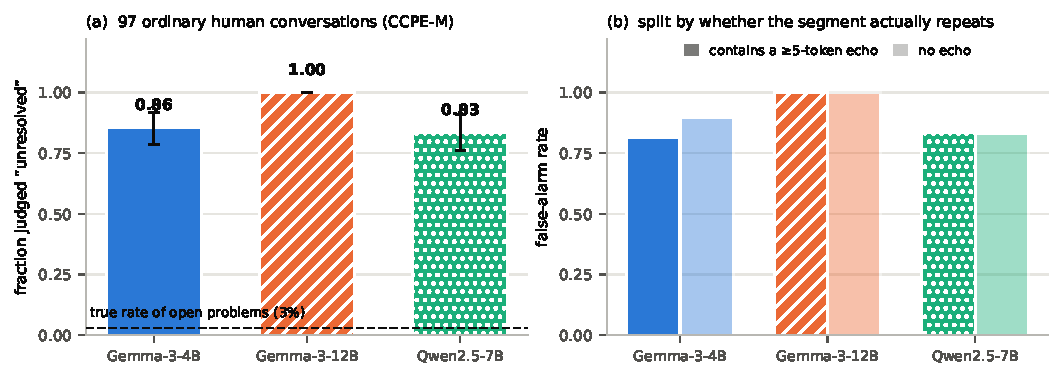
\includegraphics[width=\columnwidth]{fig1_overattribution.pdf}
\caption{Ordinary human conversation, judged. On 97 CCPE-M segments annotated \emph{resolved},
models call $84$--$100\%$ unresolved (a), and the rate does not depend on whether the segment
actually repeats (b). Bars are family-clustered bootstrap $95\%$ intervals.}
\label{fig:over}
\end{figure}

\begin{figure}[t]
\centering
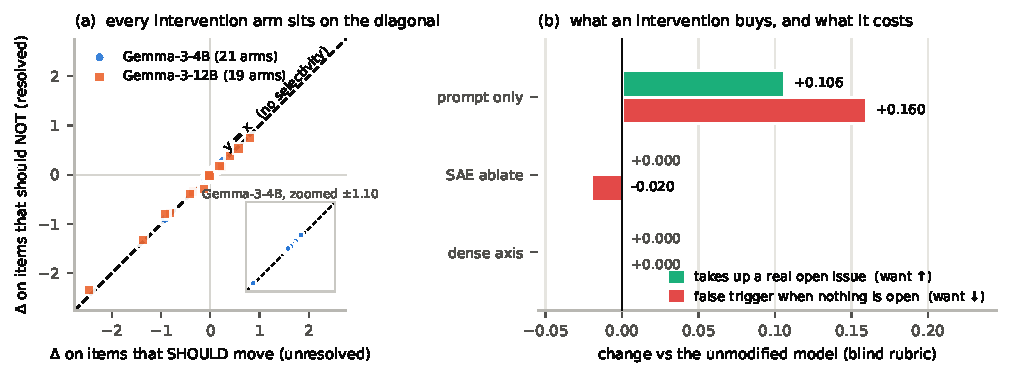
\includegraphics[width=\columnwidth]{fig2_selectivity.pdf}
\caption{No intervention is selective. (a) Every arm shifts the conditions that should move and the
conditions that should not by the same amount. (b) Blind rubric: the representational interventions
change nothing; the prompt buys a small gain at a larger cost in false triggers.}
\label{fig:sel}
\end{figure}

\section{Discussion and limitations}
\label{sec:discussion}

The prerequisite does not hold. Three instruction-tuned models, across two families and a $1.7\times$
scale range, fail to distinguish an open communication problem from a benign repetition on data
where repetition is uninformative by construction; they are beaten by a character $n$-gram model;
and they label almost all ordinary human conversation as problematic. For an
interaction-derived health signal this is the damaging failure mode, because a near-ceiling false
positive rate carries no information about the speaker while looking like a detection.

The mechanistic picture is a null with adequate controls rather than an absence of evidence: the
state is not linearly readable beyond surface statistics at a pre-registered layer, and 40
intervention arms with matched random-direction, competing-axis, random-feature and
reconstruction controls produce no selectivity at all. We therefore describe this as a causal
\emph{audit}; we do not claim a circuit, and the feature rankings are correlational.

\textbf{Limitations.} (i) The construct is an observable interaction state in ordinary task
dialogue. Nothing here measures cognition, decline or diagnosis; CCPE-M carries no cognitive-state
annotation and is not a healthy control group. (ii) Our corpus leaks: 9 of 19 surface features
separate the labels at the paired level, so every representational claim is an
incremental-over-surface claim. (iii) Annotation is LLM-assisted, not human and not clinical.
(iv) With ${\sim}25$ families per evaluation split we can exclude large selectivity effects but not
effects below ${\sim}0.15$ paired accuracy. (v) Two model families; SAE analyses require released
SAEs and so cover Gemma-3 only. (vi) Interventions act on the prompt pass; multi-turn dynamics, and
the feedback loop by which a model's reply changes the next user turn, are out of scope and are a
natural next step.

\section*{Reproducibility}
The corpus, the frozen splits and intervention configurations (write-protected, each carrying a
SHA-256 of the development evidence it was derived from), the acceptance-check suite, and a
stage-gate log recording every decision---including the two that were initially wrong---will be
released.

\begin{thebibliography}{00}
\bibitem{ngo2026} A. Ngo, N. Rollet, C. Pelachaud, and C. Clavel, ``Human vs LLM in conversational
repair annotation: a new resource and comparative study,'' in \emph{Proc. 15th Language Resources
and Evaluation Conference (LREC)}, Palma de Mallorca, 2026.
\bibitem{assistantaxis} Anthropic, ``The Assistant Axis,'' 2026. [Online]. Available:
\url{https://www.anthropic.com/research/assistant-axis}
\bibitem{clarifysae} ClarifySAE: sparse-autoencoder steering of clarification behaviour, 2026.
[Online]. Available: \url{https://github.com/sn0rkmaiden/clarifySAE-steering}
\bibitem{maira2sae} K. Bouzid, S. Bannur, F. Meissen, D. C. de Castro, A. Schwaighofer,
J. Alvarez-Valle, and S. L. Hyland, ``Insights into a radiology-specialised multimodal large
language model with sparse autoencoders,'' Actionable Interpretability Workshop, ICML, 2025.
arXiv:2507.12950.
\bibitem{cast} J. Mu and G. Chen, ``Making clinical language models auditable: concept-guided
fine-tuning for robust prediction,'' 2026. arXiv:2608.27397.
\bibitem{ccpem} F. Radlinski, K. Balog, B. Byrne, and K. Krishnamoorthi, ``Coached conversational
preference elicitation: a case study in understanding movie preferences,'' in \emph{Proc. SIGDIAL},
2019.
\bibitem{gemma3} Gemma Team, Google DeepMind, ``Gemma 3 technical report,'' 2025.
\bibitem{gemmascope} Google DeepMind, ``Gemma Scope 2: sparse autoencoders for Gemma 3,'' 2026.
[Online]. Available: \url{https://huggingface.co/google/gemma-scope-2-4b-it}
\bibitem{qwen25} Qwen Team, ``Qwen2.5 technical report,'' 2024. arXiv:2412.15115.
\end{thebibliography}

\end{document}
